\section{Implementation}
\subsection{General implementation}

	
\subsection{Map and flower patch quality}
	For the environment, two maps are used. One map indicates which flower type grows at a given integer location %TODO
\subsection{Hives}
\subsection{Scouts}
	\subsubsection{Random walk}
		\begin{figure}
			\centering
			\scalebox{.75}{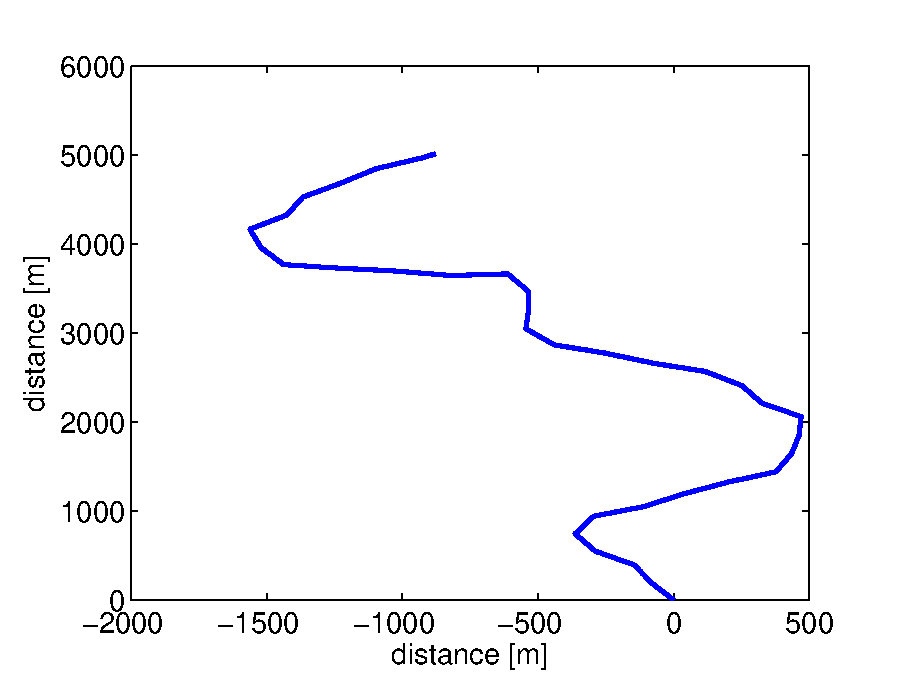
\includegraphics{data/random_walk.eps}}
			\caption{\textit{Example of a random walk executed by a scout bee.}}
			\label{fig:randomWalk}
		\end{figure}
	\subsubsection{Bresenham line algorithm}
		\begin{figure}
			\centering
			\scalebox{.75}{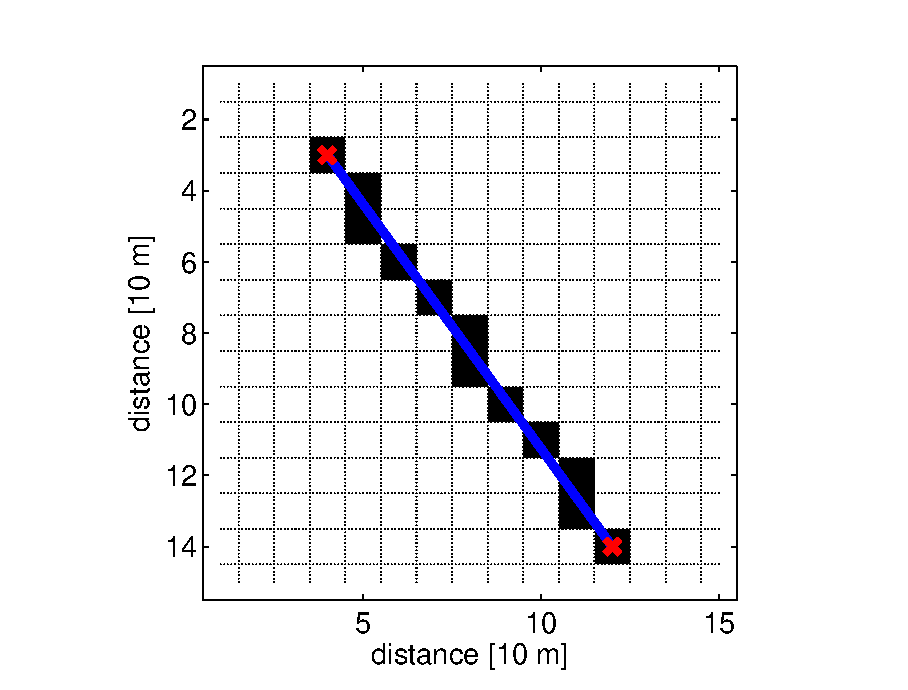
\includegraphics{data/bresenham.eps}}
			\caption{\textit{Example of Bresenham's line algorithm with map and path segment.}}
			\label{fig:bresenham}
			% SEE: http://en.wikipedia.org/wiki/Bresenham's_line_algorithm
		\end{figure}
		As the scout bees pass a distance of $v \cdot \Delta t$, respectively $\sqrt{(v_x \cdot \Delta t)^2 + (v_y \cdot \Delta t)^2}$ for a velocity $v$ and time step $\Delta t$ in every iteration step, multiple field are being passed at once. In order to check all fields between the last and current iteration step, the Bresenham line algorithm is used. With this method, all integer coordinates between two given points on the map are reported back. Afterwards, every obtained point can be checked against the current quality- and type map of the environment simulation.
		For this simple algorithm, a pre-existing implementation is used \cite{MVTB}, appendix \ref{chap:MATLAB_bresenham}. Figure \ref{fig:bresenham} is an example on a 15x15 map with coordinates $(x = 4, y = 3)$ to $(x = 12, y = 14)$ and reported points (black boxes).
\subsection{Foragers}
	\subsubsection{Path optimization}
		\begin{figure}
			\centering
			\scalebox{.75}{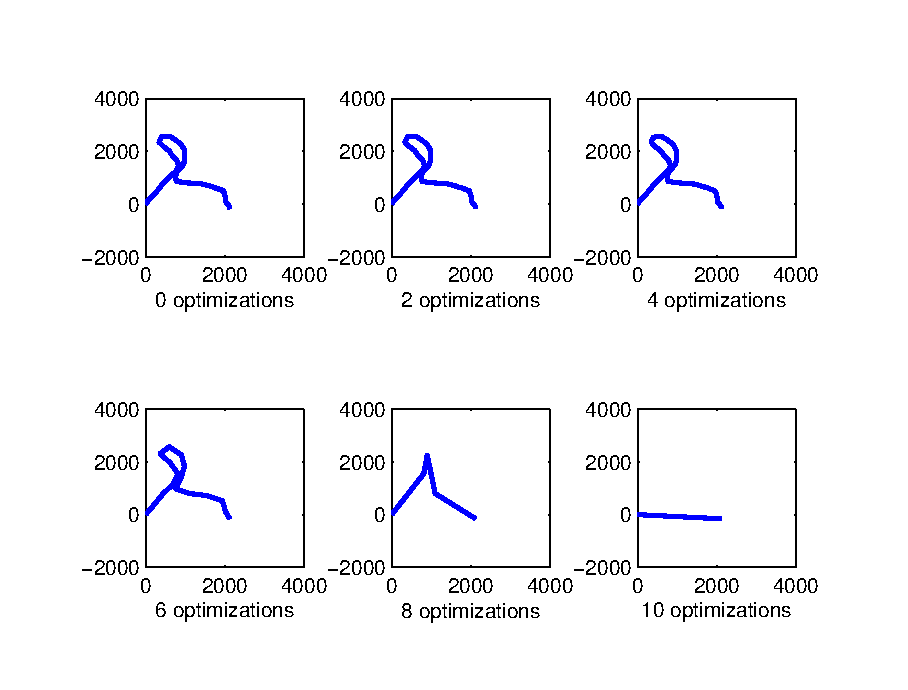
\includegraphics{data/optimization.eps}}
			\caption{\textit{Example of path optimization used to short cut the path to flower patches.}}
			\label{fig:pathOptimization}
		\end{figure}